
% Drawing angles using the PG 3.0 angles and quotes libraries
% Author: Paul Gaborit
\documentclass[tikz,border=10pt]{standalone}
%%%<
\usepackage{verbatim}
%%%>
\begin{comment}
:Title: Drawing angles using the PG 3.0 angles and quotes libraries
:Tags: Angles;Quotes;Geometry;Mathematics;PGF 3.0
:Author: Paul Gaborit
:Slug: angles-quotes

PGF 3.0 brings a new library for drawing angles. A pic type angle=a--b--c
adds a drawing of an angle to the current path. It consists of a "sector"
or "wedge" or "slice" whose pointed end is at point b and whose straight
sides lie on the lines from b to A and from B to C. You can specify
radius and eccentricity.

Another new library "quotes" is providing a quote syntax for labels, pins,
edge nodes, and pic texts. You can use a simple string "text" or a string with
options, such as node["text" {red, draw, thick}] to achieve an effect like
node[label={[red,draw,thick]text}] with less writing and more readability.

This code was written by Paul Gaborit and published on TeX.SE.
\end{comment}

\usetikzlibrary{quotes,angles}
\usetikzlibrary {arrows.meta}

\begin{document}
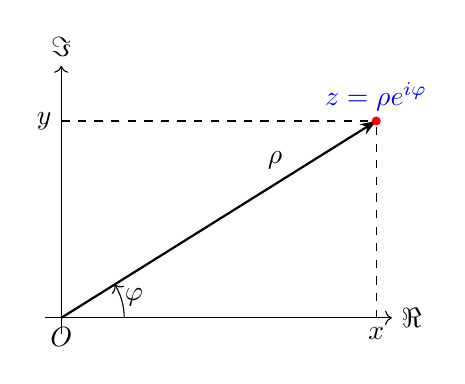
\begin{tikzpicture}

  \path (0,0) coordinate (origin);
  \path (4, 0) coordinate (x) ;
  \path (0, 2.5) coordinate (y) ;
  \path (4, 2.5) coordinate (z);
  \path (2.5, 2) coordinate (rho);

  \draw[->] (-0.2,0) --(4.2,0) node[right] {$\Re$};
  \draw[->] (0,-0.2) --(0,3.2) node[above] {$\Im$};
  \draw[solid, text=blue, thick, -{Stealth[length=2mm]}] (origin) -- (z) node[above] {$z=\rho e^{i\varphi}$};
  \draw[text=red, dashed]  (x) --(z) node[above]  {};
  \draw[text=red, dashed] (y) --(z) node[above] {};

  \node at (origin) [below] {$O$};
  \node at (x) [below ]{$x$};
  \node at (y) [left ]{ $y$};
  \node at (rho) [right] {$\rho$};
  \draw[color=red, fill=red] (z) circle (0.05);

  \draw pic["$\varphi$",draw, ->, angle eccentricity=1.2, angle radius=0.8cm]{angle = x--origin--z};

\end{tikzpicture}
\end{document}
